\subsection{Esempi di Adversarial Machine Learning}
In questa sezione andremo a vedere alcuni esempi presenti in letteratura di \textit{Adversarial Attacks} contro sistemi di Machine Learning per malware detection in Android.\\

Il metodo proposto da Papernot et al., \textit{Jacobian-based Saliency Map Attack} (JSMA) \cite{8672711}, utilizza le \textit{forward derivatives} del modello di classificazione per trovare la perturbazione ottima per la creazione di un adversarial sample. Grosse et al. lo hanno applicato al campo di Malware Detection riuscendo a raggiungere un \textit{misclassification rate} dell'\(84\%\).

Carlini \& Wanger hanno creato un modello di attacco \textit{optimization-based}, conosciuto anche come \textit{CW Attack}\cite{8672711}, che riesce a degradare le performance di classificazione di un modello raggiungendo un \textit{success rate} anche del \textit{100\%}. Chen et al. hanno ideato un attacco contro \textit{MaMadroid} e \textit{Drebin} basato su \textit{CW} e \textit{JSMA}. Il loro attacco genera \textit{adversarial sample} aggiungendo \textit{feature} binarie al codice del malware, raggiungendo un \textit{success rate} del \(100\%\) quando si ha a disposizione il modello ed i suoi parametri (\textit{withe box attack}).

Goodfellow et al. hanno introdotto \cite{8672711} l'utilizzo delle \textit{Generative Adversarial Networks} (GANs) per generare \textit{adversarial sample} partendo da \textit{noise vector}. La loro idea è stata estesa da Hu et al. per generare \textit{adversarial sample} contro malware detector di Android (\textit{black box attack}). Questa metodologia raggiunge il \(100\%\) di \textit{success rate}, senza però considerare una soglia massima di modifiche applicabili al codice del malware.

Shahpasand et al.\cite{8672711} migliorano l'idea di Goodfellow et al., introducendo una soglia (\textit{threshold}) per il livello massimo di distorsione applicabile al codice del malware originale. 

\subsubsection{Metodo di Shahpasand et al.}
Il metodo proposto da Shahpasand et al.\cite{8672711} si basa sulla tecnica dell'\textit{evasion} per cercare di eludere il classificatore e indurlo a catalogare Malware come file benigni. Il loro obbiettivo è quindi quello di generare \textit{adversarial sample}, partendo dal codice originale di un malware, per ingannare il Malware Detector. In modo più formale:

Sia \(X = \{0, 1\}^m\) il \textit{feature space}, con \(m\) il numero delle \textit{feature}, dove \(x \in X\) indica la presenza dell'\textit{i-esima} \textit{feature} in una parte di codice. Il classificatore deduce \(f : X \to Y\) dal dominio \(X\) alle etichette \textit{benigno} o \textit{maligno} \(y \in \{0, 1\}\). Dato un malware \(x\) con la sua \textit{true label} \(f(x) = 1\), l'attaccante punta a generare un \textit{adversarial sample} \(x' = x + \delta\) che risulti avere  \(f(x') = 0\).\\
\\
Utilizzano quindi una \textit{GAN} per cercare la perturbazione \(\delta\) ottimale da aggiungere al malware. L'architettura generale viene illustrata nella seguente figura:

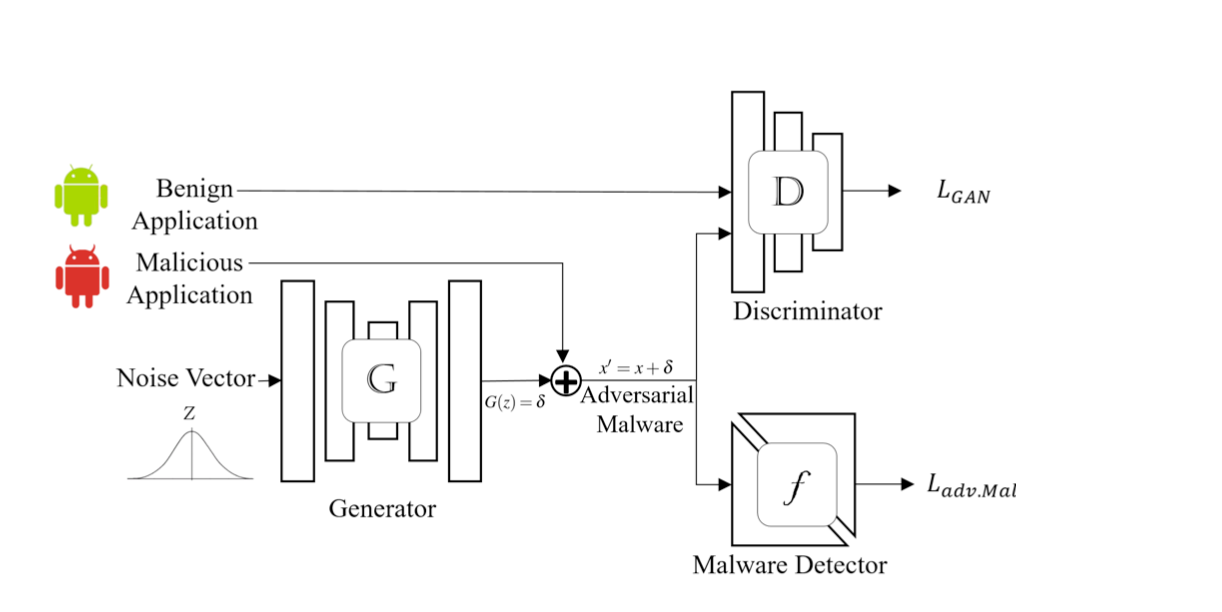
\includegraphics[scale=0.6]{model.png}

Il \textit{Generator G} prende in input un \textit{noise vector} \(z\) e genera la perturbazione ottima \(G(z) = \delta\).
Il \textit{Discriminator} usa come input un \textit{sample} \textit{benigno} e il \textit{sample} del malware distorto per poter diversificare il sample benigno dall'\textit{adversarial malware}. Il \textit{Discriminator} migliora la perturbazione aumentando la \textit{loss} del \textit{Generator} se l'\textit{adversarial malware} è distinguibile dal \textit{sample benigno}.\\
Queste due componenti sono \textit{feed-forward neural network} che vengono allenate in maniera alternata in modo da ottimizzare la \textit{min-max loss function}.\\
Utilizzano una loro \textit{loss function} formata da due elementi principali:

\begin{itemize}
    \item \textbf{L\textsubscript{GAN} function}\cite{8672711}, definita come: 
            \[
                L_{GAN} = {}_{x \sim P_{Benign}} logD(x) \ + \
                          {}_{x \sim P_{Malware}, \ z \sim P_{z}(z)} log(1 - D(x + G(z))) \ \ 
                          s.t.|G(z)| < c
            \]
            
            dove \(D(x)\) è la probabilità che il \textit{sample} \(x\) derivi da un software benigno, \(L_{GAN}\) indica la necessità di avere un \textit{Adversarial Malware} il più simile possibile ad uno \textit{sample} benigno, avendo una distorsione che non superi una certa soglia \(c\). \(|G(z)|\) è il numero di \textit{feature} aggiunte dalla perturbazione, se questo è troppo elevato rende immediatamente evidente l'attacco e potrebbe essere molto dispendioso applicare le modifiche al codice (in termini di costi e tempo).
    
    \item \textbf{L\textsubscript{adv.Mal} function}\cite{8672711}, definita come: 
            \[
                L_{adv.Mal} = {}_{x, z} l_f(x + G(z), 0)
            \]
            
            dove la classe \textit{Benigna}, con etichetta 0, è scelta come bersaglio per un \textit{adversarial sample} \(x + G(z)\) contro il Malware Detector \(f\) allenato con la \textit{loss function} \(l_f\). % \textbf{note by Alina: il classificatore sarebbe il malware detector?}
\end{itemize}

La funzione utilizzata da Shahpasand et al. è quindi:

\[
    L = \alpha L_{GAN} + (1 - \alpha )L_{adv.Mal}
\]



dove il primo termine indica una funzione che forza la GAN a generare un \textit{adversarial sample} simile ad un \textit{benign sample} e il secondo è un \textit{adversarial malware sample} con un alto \textit{misclassification rate}.\\
\\
Per la fase di training e testing, gli autori utilizzano il dataset \textit{Drebin Android} che contiene \(129.013\) applicazioni, in formato \textit{APK}, di cui \(5.560\) sono malware. Ogni applicazione Android include il \textit{Manifest} ed il \textit{dexcode}, che sono le principali risorse da cui vengono estratte le \textit{feature}. Queste vengono catalogate in 8 \textit{feature set} che saranno poi utilizzate per la classificazione.\\

\begin{center}
    \begin{tabular}{ll}
    \cline{1-2}
    \multicolumn{1}{c}{\textit{manifest}} & \multicolumn{1}{c}{\textit{dexcode}} \\
    \cline{1-2} 
        Hardware components & Restricted API calls\\ [0.5ex]
        Requested permissons & Used permission  \\ [0.5ex]
        Application components & Suspicious API calls \\ [0.5ex]
        Filtered intents & Network addresses \\ [0.5ex]
    \cline{1-2}
    \end{tabular}
    \captionof{table}{Feature Set del dataset Drebin Android.}
\end{center}
\ \\
La \textit{GAN} è stata allenata contro le seguenti tipologie di classificatori (tutti allenati con le impostazioni di default proposte dalla libreria \say{scikit-learn} di Python: \(80\%\) del dataset come \textit{training set}):

\begin{itemize}
    \item Support Vector Machine (SVM)
    \item Neural Networks (NN)
    \item Random Forest (RF)
    \item Logic Regression (LR)
\end{itemize}

Il risultato è stato che quasi tutti i classificatori sono molto vulnerabili a questo tipo di attacco: quasi il \(99 \%\) di \textit{success rate} contro le Neural Network e Logic Regression e fino all'\(87 \%\) contro le Support Vector Machine. Le Random Forest sono state le uniche più resistenti, con un \textit{success rate} non superiore al \(52 \%\).

\subsubsection{Metodo di Xiao Chen et al.}
Xiao Chen et al.\cite{hiv} propongono una metodologia di attacco \textit{black-box}, basata su \textit{CW} e \textit{JSMA}, contro due diverse tipologie di Malware Detector che rappresentano lo \textit{state-of-the-art} nel campo: \textit{MaMaDroid}, basato sulle \textit{Random Forest} e Drebin, basato su \textit{Support Vector Machine}.
Il meccanismo su cui si basa il loro attacco consiste nel trovare la perturbazione ottima da applicare all'archivio \textit{APK} per portare i classificatori ad etichettare file maligni come benigni.
Propongono anche un \textit{framework} che, in automatico senza alcun intervento umano, è in grado di decomprimere l'\textit{APK}, aggiungere le modifiche ai file \textit{.dex} e ricompattare il tutto formando un nuovo \textit{APK}. Dai risultati presentati nel paper è possibile notare come i loro \textit{Adversarial Sample} riducono la precisione dal \(96\%\) al \(1\%\) per MaMaDroid\cite{hiv} e dal \(97\%\) al \(1\%\) per Drebin\cite{hiv}.\\
\\
\textbf{Attacco a MaMaDroid}\\
La creazione di \textit{Adversarial Sample} contro MaMaDroid avviene con l'aggiunta, il meno invasiva possibile, di chiamate API al codice \textit{smali}.
Il codice \textit{smali} è il risultato di un operazione effettuata su un file \textit{.dex}, un file binario, per renderlo più facilmente interpretabile e modificabile.\\

\begin{lstlisting}[caption=Esempio di formati dex e smali. La riga 1 rappresenta il codice originale scritto in Java. La riga 2 è il contenuto dello stesso codice compilato in formato dex. La riga 3 è il codice smali ottenuto dalla conversione del file dex.]
    int x = 42;         // Java
    13 00 2A 00         // .dex
    const/16 v0, 42     // smali
\end{lstlisting}
\ \\
Utilizzano delle versioni appositamente modificate degli algoritmi \textit{CW} e \textit{JSMA} per calcolare il numero di perturbazioni (chiamate a funzioni) da aggiungere al codice. %% per allungare il brodo posso metterci lo pseudocodice incomprensibile
Il tutto si basa su come MaMaDroid calcola il \textit{feature space} dell'app che deve analizzare. Aggiungendo un determinato numero di chiamate a API che partono da una specifica funzione chiamata \textit{caller} ad un'altra chiamata \textit{callee}, riescono ad alterare il valore del \textit{feature space} inducendo il classificatore in una predizione errata. Propongono due versioni di questa procedura, una chiamata \textit{Semplice} e l'altra \textit{Sofisticata}. Di seguito una breve descrizione della \textit{Semplice}.\\

La strategia \textit{Semplice} inganna MaMaDroid aggiungendo specifiche classi nell'archivio \textit{APK} e invocandone i metodi all'interno di \textit{onCreate()} nella \textit{MainActivity}, per fargli estrarre un errato \textit{feature vector}. Questo viene calcolato prendendo tutte le chiamate API dal file \textit{classes.dex} e le converte nelle relative famiglie o pacchetti. Per esempio, una classe \textit{MyClass} (da noi definita) contenuta all'interno di un pacchetto \textit{android.os.mypack} (da noi definito) e la classe di sistema \textit{StorageManager} presente all'interno del pacchetto di sistema \textit{android.os.storage}, verranno ambedue convertite come famiglia \textit{android} o come pacchetto \textit{android.os}. Xiao Chen et al. sfruttano questa debolezza per indurre MaMaDroid ad effettuare classificazioni errate. È bene notare che l'aggiunta di queste chiamate non comporta alcuna modifica alle funzionalità originali del malware ed è possibile aggiungerne un numero arbitrario tramite l'utilizzo di un semplice script.\\

\begin{lstlisting}[language=Java, label={lst:label}, caption=Esempio di classe ideata da Xiao Chen et al.\cite{hiv} per sfruttare la debolezza del calcolo del \textit{feature vector} di MaMaDroid]
    package android.os.mypack
    
    public class Myclass {
        public static void callee() {} 
        public static void caller() {
              callee();
              callee();
        }
    }
\end{lstlisting}

\begin{lstlisting}[caption=Equivalente del codice di \textit{Listing \ref{lst:label}} in smail]
    .class public Landroid/os/mypack/Myclass; 
    .source "Myclass.java"
    
    .method public static callee()V 
        .locals 0
        return-void .end method

    .method public static caller()V 
        .locals 0
        .line 6 invoke-static {},
            Landroid/os/mypack/Myclass;->callee()V 
        return-void
    .end method
\end{lstlisting}
\ \\

\pagebreak

\begin{figure}[h!]
  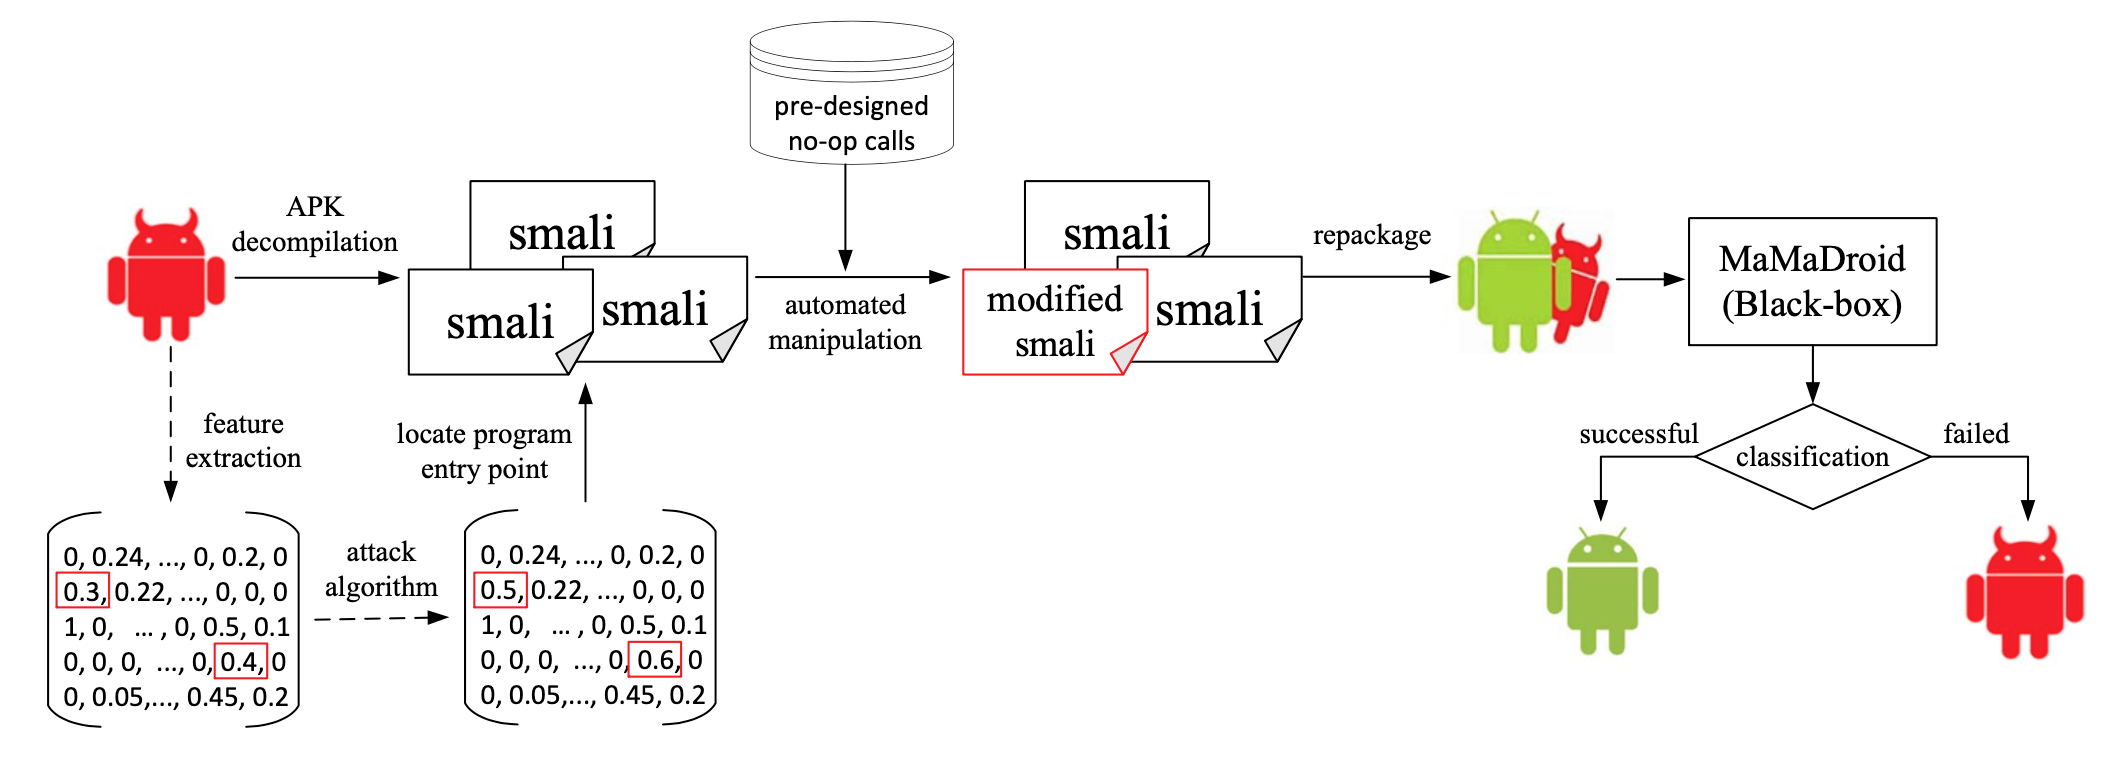
\includegraphics[scale=0.4]{aml_vs_md/imgs/chen_mamadroid.png}
  \caption{Xaio Chen et al. vs MaMaDroid}
  Questo diagramma mostra il funzionamento del metodo di Xiao Chen et al. contro MaMadroid. Le linee tratteggiate indicano il processo di attacco, le altre linee indicano il processo di manipolazione del file APK
\end{figure}

\ \\
Per la fase di testing hanno utilizzato MaMaDroid con le impostazioni di default fornite dagli autori e come dataset lo stesso utilizzato per MaMaDroid: un set di 5.879 software benigni e 5.560 software maligni.
Dagli esperimenti che hanno condotto si evince che questo attacco ha un \textit{success rate} che va dal \(56\%\)\cite{hiv} fino al \(96\%\)\cite{hiv}.\\
\ \\
\textbf{Attacco a Drebin}\\
Anche per attaccare Drebin sfruttano il modo in cui il sistema calcola il \textit{feature vector} con cui rappresentare il potenziale malware. Per ottenerlo, Drebin effettua una \say{scansione lineare} sui file \textit{smali} e \textit{AndroidManifest.xml} andando a cercare solo la presenza di stringhe particolari, come il nome di chiamate API, senza andare a controllare se effettivamente le chiamate vengono eseguite. La loro strategia è quindi di andare ad aggiungere il codice (perturbazione) ai file \textit{smali}, sotto forma di metodi o funzioni, senza però inserire l'istruzione per l'invocazione o esecuzione.

\begin{lstlisting}[caption=Esempio di perturbazione che verrà aggiunta nei file smali.]
    .method private addSuspiciousApiFeature()V .locals 1
    const-string v0, "phone" .line 17
    invoke-virtual {p0, v0},
          La/test/com/myapp/MainActivity;->
          getSystemService(Ljava/lang/String;)
          Ljava/lang/Object;
       move-result-object v0
       check-cast v0,
    Landroid/telephony/TelephonyManager; return-void
    .end method
\end{lstlisting}
\ \\
Per trovare la perturbazione ottima utilizzano l'attacco JSMA che, tramite la matrice Jacobiana, riesce ad individuare la \textit{feature} più influente da modificare per ogni iterazione. Il processo si ferma quando l'\textit{adversarial sample} creato viene \textit{misclassificato} oppure non si raggiunge la soglia massima di modifiche permesse. La matrice Jacobiana viene calcolata come: 

\[
    J_F(X) = [ \frac{\partial F(x)}{\partial X} ] = [ \frac{\partial F_j(X)}{\partial x_i} ]_{i \in 1 \ldots n, \ j \in 0, 1}
\]

dove \(X\) è il \textit{feature vector binario} per \textit{Drebin} ed \(i\) è il risultato della classificazione (\(i = 1\) per indicare un malware).\\
\\
Per condurre gli esperimenti hanno utilizzato lo stesso dataset dell'attacco a MaMaDroid e dai risultati si può notare come questa metodologia raggiunge un \textit{success rate} fino al \(99\%\)\cite{hiv}.

\subsubsection{Metodo di Xiaolei Liu et al.}
Xiaolei et al.\cite{iot} propongono una metodologia di attacco \textit{black-box} con utilizzo di \textit{Algoritmi Genetici} contro Malware Detection per sistemi \textit{IoT} basati su Android, chiamato \textit{TLAMD}.\\
\\
Il loro obbiettivo è sempre quello di portare un Malware Detector a classificare un file maligno come benigno. L'approccio che utilizzano è quello di andare ad inserire \textit{permission feature}\cite{iot} solo all'interno del file \textit{AndroidManifest.xml} per evitare di alterare il funzionamento del codice del malware stesso e rendere più semplice applicare la modifica. Per aggiungere una sicurezza in più nel non alterare il corretto funzionamento del software andranno solo ad aggiungere elementi e mai a toglierli. Il numero di \textit{feature} aggiunte rimane comunque importante: minore sarà la perturbazione meglio è, ovvero, minori saranno le modifiche al \textit{file manifest} meglio è. Per far ciò applicano un algoritmo genetico che gli permette di trovare il minor numero di perturbazioni \(\delta\) da applicare.

\begin{lstlisting}[caption=Pseudocodice per la generazione di un \textit{Adversarial Sample}\cite{iot}, mathescape=true]
    Require: Popluation Size pop_size 
        $\delta$ $\leftarrow$ initialization()
        for i=0 $\rightarrow$ pop_size do
            Pi $\leftarrow$ Crossover_Operator()
            Pi $\leftarrow$ Mutation_Operator() 
            Compute $\rightarrow$  S($\delta$)
            if F(X + $\delta$) > 1 - F(X + $\delta$) then
                Continue
            else
                Output $\rightarrow$ $\delta$
            end if
        end for
\end{lstlisting}
\ \\
L'algoritmo per la creazione degli \textit{Adversarial Sample} può essere riassunto nei seguenti punti\cite{iot}:

\begin{enumerate}
    \item \textbf{Generazione casuale} della popolazione \(\delta\) composta dalle varie \textit{permission feature}.
    \item \textbf{Individuazione} della \textit{fitness function} che servirà per trovare una soluzione ottima per indurre il classificatore ad una predizione errata.
    \item \textbf{Esecuzione} delle operazioni di \textit{Mutazione}
    \item \textbf{Generazione} di una \textbf{nuova popolazione} partendo dalle operazioni di mutazione del punto precedente e ritornare al punto 2. Se il numero prestabilito di iterazioni viene raggiunto, l'algoritmo termina.
\end{enumerate}

\begin{figure}[H]
  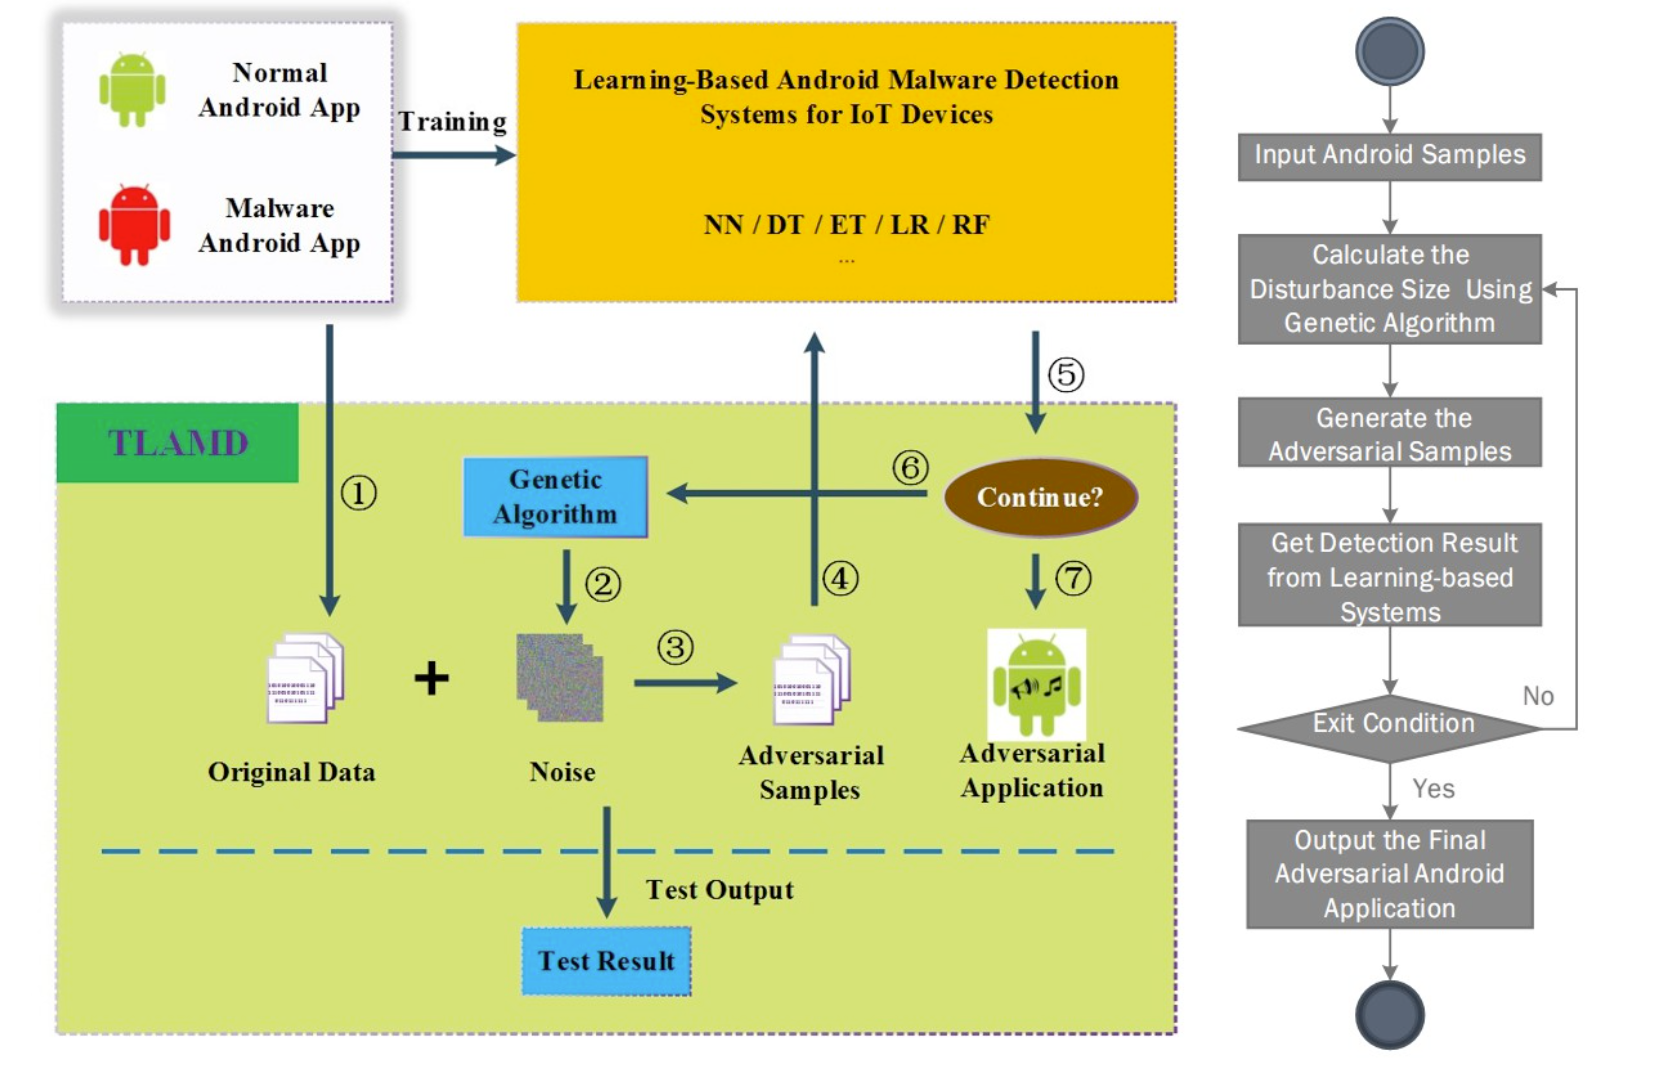
\includegraphics[scale=0.5]{aml_vs_md/imgs/iot.png}
  \caption{Funzionamento di TLAMD}
  Questo schema illustra il funzionamento dell'algoritmo per la generazione di Adversarial Sample\cite{iot}. \textcircled{1} Codice originale del Malware come input. \textcircled{2} Calcolo della perturbazione. \textcircled{3} Generazione dell'\textit{Adversarial Sample}. \textcircled{4} Valore di ritorno del classificatore. \textcircled{5} Controlla se la condizione di uscita è verificata. \textcircled{6} Se non lo è, viene calcolata nuovamente la perturbazione con l'algoritmo genetico. \textcircled{7} Se si, viene restituito in output il nuovo Malware.
\end{figure}
\ \\
Per verificare l'efficacia del loro attacco, hanno allenato 5 diversi modelli di classificatori tra cui \textit{Logic Regression} (LR), \textit{Decision Tree} (DT) e \textit{Fully Connected Neural Networks} (NN), con lo stesso dataset utilizzato per \textit{Drebin}. Solo quando questi raggiungeranno un determinato valore di \textit{Accuracy} potranno essere attaccati.\\

\begin{center}
    \begin{tabular}{l|c}
        \multicolumn{1}{c}{\textbf{Modello}} & \multicolumn{1}{c}{\textbf{Accuracy}}  \\ [0.5 em]
        NN (Neural Network) & 99.83\% \\ [0.5 em]
        LR (Logic Regression) & 99.45\% \\ [0.5 em]
        DT (Decision Tree) & 99.86\% \\ [0.5 em]
        RF (Random Forest) & 99.92\% \\ [0.5 em]
        ET (Extreme Tree) & 99.96\% \\
    \end{tabular}
    \captionof{table}{La tabella mostra sulla sinistra i vari tipi di modelli utilizzati e sulla destra i valori la loro \textit{Accuracy} \cite{iot}}
\end{center}
\ \\
Hanno generato Adversarial Sample per ogni tipologia di modello ed hanno verificato che il loro metodo risulta essere molto efficace: il \textit{success rate} è sempre sopra l'\(80\%\)\cite{iot} e molto spesso si avvicina al \(100\%\)\cite{iot}. Le \textit{Neural Network} (NN) risultano estremamente vulnerabili (con un \textit{success rate} del \(100\%\), invece le \textit{Extreme Tree} (ET) sono leggermente più resistenti delle altre (con un \textit{success rate} di circa l'\(83\%\)).

